\title{Aula 2 - Sistemas de Numeração Digital}



\begin{frame}
    \titlepage
\end{frame}



\begin{frame}{Sistemas de Numeração Digital}
    \begin{itemize}
        \item \textbf{Panorama Geral:} Na tecnologia digital, utilizamos diferentes bases numéricas para finalidades específicas.
        \item \textbf{Bases mais usadas:}
              \begin{itemize}
                  \item \textbf{Decimal (Base 10)}
                  \item \textbf{Binário (Base 2)}
                  \item \textbf{Octal (Base 8)}
                  \item \textbf{Hexadecimal (Base 16)}
              \end{itemize}
    \end{itemize}

\end{frame}

\begin{frame}{Sistema Decimal (Base 10)}
    \begin{itemize}
        \item \textbf{Símbolos:} Composto por 10 dígitos: $\{0, 1, 2, 3, 4, 5, 6, 7, 8, 9\}$.
        \item \textbf{Origem:} Evoluiu do uso dos dez dedos das mãos para contagem
        \item \textit{dígito} vem do latim \textit{digitus}, "dedo".
        \item \textbf{Sistema Posicional:} O valor de um dígito depende da sua posição no número.
    \end{itemize}
\end{frame}


\begin{frame}{Contagem decimal}
    \begin{center}
        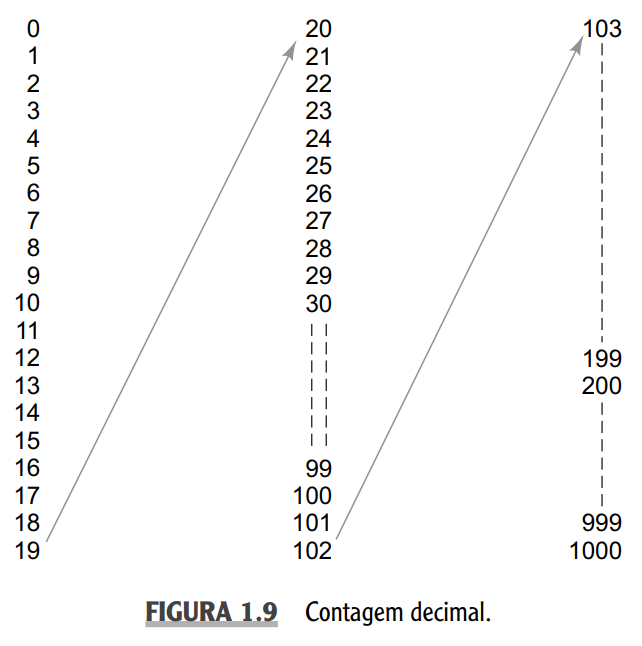
\includegraphics[width=0.7\textwidth]{Figuras/contagem-decimal.png}

    \end{center}


\end{frame}

\begin{frame}{Sistema Decimal (Base 10)}
    \begin{exampleblock}{Exemplo: Número 453}
        \centering
        \begin{tabular}{c c c}
            \textbf{4}        & \textbf{5}       & \textbf{3}        \\
            Centenas ($10^2$) & Dezenas ($10^1$) & Unidades ($10^0$) \\
        \end{tabular}
    \end{exampleblock}

    \begin{itemize}
        \item \textbf{MSD (Most Significant Digit):} O dígito de maior peso (neste caso, o \textbf{4}).
        \item \textbf{LSD (Least Significant Digit):} O dígito de menor peso (neste caso, o \textbf{3}).
    \end{itemize}

\end{frame}

\begin{frame}{Representação Formal do Sistema Decimal}
    \begin{itemize}
        \item \textbf{Estrutura Genérica:} Qualquer número decimal pode ser escrito como uma sequência de dígitos $d$ em relação à vírgula:
              $$d_n d_{n-1} \dots d_1 d_0 , d_{-1} d_{-2} \dots d_{-k}$$
    \end{itemize}

    \begin{block}{Expansão Polinomial}
        O valor real é a soma de cada dígito multiplicado pelo peso de sua posição:
        $$Valor = \sum_{i=-k}^{n} d_i \times 10^i$$
    \end{block}

    \begin{itemize}
        \item \textbf{Componentes:}
              \begin{itemize}
                  \item $d_i$: O algarismo na posição $i$ (de 0 a 9).
                  \item $10^i$: O peso (base elevada à posição).
                  \item $n$ e $k$: Número de dígitos inteiros e fracionários, respectivamente.
              \end{itemize}
    \end{itemize}

    \vspace{0.2cm}
    \centering
    \textit{Essa mesma lógica será aplicada ao sistema binário, apenas trocando a base 10 por 2.}
\end{frame}

\begin{frame}{Formalização da Notação Posicional}
    \begin{itemize}
        \item \textbf{Definição:} A posição do dígito determina a potência da base pela qual ele será multiplicado.
        \item Assim, representamos infinitos valores com um conjunto finito de símbolos.
    \end{itemize}

    \begin{block}{Formalizando}
        Para definir um sistema posicional, precisamos de:
        \begin{enumerate}
            \item \textbf{Uma Base ($B$):} O número de símbolos distintos.
            \item \textbf{Conjunto de Símbolos:} Valores inteiros de $0$ até $B-1$.
        \end{enumerate}
    \end{block}



\end{frame}



\begin{frame}{Representação Genérica em Base $B$}
    Com a base ($B$) e o conjunto de símbolos definidos, temos:

    \begin{itemize}
        \item \textbf{Sequência de dígitos:} $s = b_i$, para $i \in -k \dots n$.
        \item \textbf{Cálculo do Valor:}
    \end{itemize}

    \begin{block}{Fórmula Geral}
        $$ \text{Valor} = \sum_{i=-k}^{n} b_i B^i $$
    \end{block}

    \begin{itemize}
        \item \textbf{Expansão da Soma:}
              {\small
                  $$ b_n B^n + b_{n-1} B^{n-1} + \dots + b_0 B^0 + b_{-1} B^{-1} + \dots + b_{-k} B^{-k} $$
              }
        \item \textbf{Convenção de Escrita:} A posição menos significativa fica sempre à direita:
              $$ b_n b_{n-1} \dots b_1 b_0 , b_{-1} \dots b_{-k+1} b_{-k} $$
    \end{itemize}
\end{frame}

\begin{frame}{Exemplo de Decomposição: Inteiros (Base 10)}
    Considere a sequência \textbf{347} na base 10. Aplicando a fórmula da soma de produtos pelo peso da posição:

    \begin{itemize}
        \item \textbf{Decomposição:}
    \end{itemize}

    $$ 3 \times 10^2 + 4 \times 10^1 + 7 \times 10^0 $$


    $$ 3 \times 100 + 4 \times 10 + 7 \times 1 = 300 + 40 + 7 $$

    \begin{itemize}
        \item \textbf{Resultado:}
    \end{itemize}

    $$ 347_{10} $$


\end{frame}

\begin{frame}{Exemplo de Decomposição: Fracionários (Base 10)}
    Considere a sequência \textbf{58,25} na base 10. Note o uso de potências negativas para os dígitos após a vírgula:

    \begin{itemize}
        \item \textbf{Decomposição:}
    \end{itemize}

    $$ 5 \times 10^1 + 8 \times 10^0 + 2 \times 10^{-1} + 5 \times 10^{-2} $$



    $$ 50 + 8 + \frac{2}{10} + \frac{5}{100} = 50 + 8 + 0,2 + 0,05 $$

    \begin{itemize}
        \item \textbf{Resultado:}
    \end{itemize}

    $$ 58,25_{10} $$
\end{frame}

\begin{frame}{Valor Posicional e Potências de 10}
    \begin{itemize}
        \item \textbf{A Vírgula Decimal:} Atua como o separador entre a parte \textbf{inteira} (potências positivas) e a parte \textbf{fracionária} (potências negativas).
        \item \textbf{Estrutura de Pesos:} Cada posição possui um peso que é uma potência de 10 ($10^n$).
    \end{itemize}

    \begin{exampleblock}{Decomposição do número 2745,214}
        $$ (2 \times 10^3) + (7 \times 10^2) + (4 \times 10^1) + (5 \times 10^0) + (2 \times 10^{-1}) + (1 \times 10^{-2}) + (4 \times 10^{-3}) $$
    \end{exampleblock}

    \begin{itemize}
        \item \textbf{Regra Geral:} Qualquer número é a soma dos produtos de cada dígito pelo seu valor posicional.
    \end{itemize}


\end{frame}

\begin{frame}{Exemplo}
    \begin{center}
        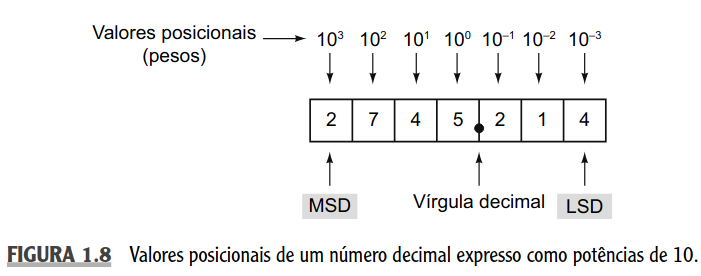
\includegraphics[width=\textwidth]{Figuras/MSDLSD.png}

    \end{center}


\end{frame}

\begin{frame}{Exercício}
    Decomponha os seguintes números decimais, considerando a notação posicional.


    \begin{enumerate}[a)]
        \item \textbf{3014}

        \item \textbf{-25,5}

        \item \textbf{10,01}


        \item \textbf{-10750}

    \end{enumerate}
\end{frame}


\begin{frame}{Exercício}
    Decomponha os seguintes números decimais, considerando a notação posicional.




    \begin{enumerate}[a)]
        \item \textbf{3014}
              \begin{itemize}
                  \item $(3 \times 10^3) + (0 \times 10^2) + (1 \times 10^1) + (4 \times 10^0)$
              \end{itemize}

        \item \textbf{-25,5}
              \begin{itemize}
                  \item $-( (2 \times 10^1) + (5 \times 10^0) + (5 \times 10^{-1}) )$
              \end{itemize}

        \item \textbf{10,01}
              \begin{itemize}
                  \item $(1 \times 10^1) + (0 \times 10^0) + (0 \times 10^{-1}) + (1 \times 10^{-2})$
              \end{itemize}

        \item \textbf{-10750}
              \begin{itemize}
                  \item $-( (1 \times 10^4) + (0 \times 10^3) + (7 \times 10^2) + (5 \times 10^1) + (0 \times 10^0) )$
              \end{itemize}
    \end{enumerate}


    \textit{Nota: O sinal é uma informação adicional à esquerda e não segue a convenção de posição/expoente.}


\end{frame}


\title{Aula 2 - Utilizando outras bases}



\begin{frame}
    \titlepage
\end{frame}


\begin{frame}{Comparativo de Bases e Símbolos}
    \begin{itemize}
        \item Seguindo a regra do intervalo $[0, B-1]$, temos os seguintes conjuntos:
    \end{itemize}

    \begin{table}[]
        \centering
        \begin{tabular}{|l|c|l|c|}
            \hline
            \textbf{Sistema} & \textbf{Base ($B$)} & \textbf{Símbolos Disponíveis} & \textbf{Intervalo} \\ \hline
            Binário          & 2                   & 0, 1                          & $0$ a $B-1$        \\ \hline
            Octal            & 8                   & 0, 1, 2, 3, 4, 5, 6, 7        & $0$ a $B-1$        \\ \hline
            Decimal          & 10                  & 0, 1, 2, 3, 4, 5, 6, 7, 8, 9  & $0$ a $B-1$        \\ \hline
            Hexadecimal      & 16                  & 0-9, A, B, C, D, E, F         & $0$ a $B-1$        \\ \hline
        \end{tabular}
    \end{table}

    \begin{block}{Convenção para Bases Maiores ($B > 10$)}
        Como não existem algarismos únicos para valores acima de 9, usamos letras:
        \centering
        \textbf{A}=10, \textbf{B}=11, \textbf{C}=12, \textbf{D}=13, \textbf{E}=14, \textbf{F}=15
    \end{block}
\end{frame}

\begin{frame}{Bases de Numeração: Base 10 (Decimal)}
    \begin{itemize}
        \item \textbf{Uso:} Base com a qual estamos familiarizados e interagimos como usuários.
        \item \textbf{Notação:}
              \begin{itemize}
                  \item Indicada pelo índice $_{10}$.
                  \item \textbf{Padrão (Default):} Se não houver indicação de base, assume-se que o número é decimal.
              \end{itemize}
    \end{itemize}

    \begin{exampleblock}{Exemplos}
        \centering
        $345$ \quad ou \quad $345_{10}$
    \end{exampleblock}
\end{frame}

\begin{frame}{Bases de Numeração: Base 2 (Binária)}
    \begin{itemize}
        \item \textbf{Uso:} Linguagem nativa dos circuitos digitais.
        \item \textbf{Notação Acadêmica:} Indicada pelo índice $_2$.
        \item \textbf{Em Programação:} Precedida pelos caracteres \texttt{0B} ou \texttt{0b}.
    \end{itemize}

    \begin{exampleblock}{Exemplos}
        \centering
        $10111_2$ \quad ou \quad \texttt{0b10111}
    \end{exampleblock}


\end{frame}

\begin{frame}{Bases de Numeração: Base 8 (Octal)}
    \begin{itemize}
        \item \textbf{Notação Acadêmica:} Indicada pelo índice $_8$.
        \item \textbf{Em Programação:}
              \begin{itemize}
                  \item Precedida por \texttt{0O} ou \texttt{0o}.
                  \item Em algumas linguagens (como C antigo), precedida apenas por \texttt{0}.
              \end{itemize}
    \end{itemize}

    \begin{exampleblock}{Exemplos}
        \centering
        $107_8$ \quad ou \quad \texttt{0o107} \quad ou \quad \texttt{0107}
    \end{exampleblock}
\end{frame}



\begin{frame}{Bases de Numeração: Base 16 (Hexadecimal)}
    \begin{itemize}
        \item \textbf{Uso:} Representação compacta de binários.
        \item \textbf{Notação Acadêmica:} Indicada pelo índice $_{16}$.
        \item \textbf{Em Programação:} Precedida pelos caracteres \texttt{0X} ou \texttt{0x}.
    \end{itemize}

    \begin{exampleblock}{Exemplos}
        \centering
        $1C7_{16}$ \quad ou \quad \texttt{0x1C7}
    \end{exampleblock}

    \begin{alertblock}{Lembrete}
        Utiliza dígitos de 0 a 9 e as letras de A a F (para representar de 10 a 15).
    \end{alertblock}
\end{frame}

\begin{frame}{Valores de 0 a 15 nas bases 2, 8, 10 e 16}
    \begin{table}[h]
        \begin{center}
            \begin{tabular}{|c|c|c|c|}
                \hline
                10 & 2    & 8  & 16 \\
                \hline
                0  & 0    & 0  & 0  \\
                1  & 1    & 1  & 1  \\
                2  & 10   & 2  & 2  \\
                3  & 11   & 3  & 3  \\
                4  & 100  & 4  & 4  \\
                5  & 101  & 5  & 5  \\
                6  & 110  & 6  & 6  \\
                7  & 111  & 7  & 7  \\
                8  & 1000 & 10 & 8  \\
                9  & 1001 & 11 & 9  \\
                10 & 1010 & 12 & A  \\
                11 & 1011 & 13 & B  \\
                12 & 1100 & 14 & C  \\
                13 & 1101 & 15 & D  \\
                14 & 1110 & 16 & E  \\
                15 & 1111 & 17 & F  \\
                \hline
            \end{tabular}
        \end{center}
    \end{table}
\end{frame}

\begin{frame}{Exercício: Contagem em Múltiplas Bases}

    Escreva os números de 0 a 20 nas seguintes bases:

    2, 5, 8, 10, 11 e 16.

    \vspace{0.3cm}
    \begin{alertblock}{Dicas!}
        \begin{itemize}
            \item Na \textbf{Base 5}, o número após o $4$ é o $10_5$.
            \item Na \textbf{Base 11}, o número $10$ é representado pela letra $A$.
        \end{itemize}
    \end{alertblock}
\end{frame}

\begin{frame}{Gabarito: Contagem de 0 a 20 em Diferentes Bases}
    \centering
    \resizebox{0.7\textwidth}{!}{
        \begin{tabular}{|c|c|c|c|c|c|}
            \hline
            \textbf{Base 10} & \textbf{Base 2} & \textbf{Base 5} & \textbf{Base 8} & \textbf{Base 11} & \textbf{Base 16} \\ \hline
            0                & 0               & 0               & 0               & 0                & 0                \\ \hline
            1                & 1               & 1               & 1               & 1                & 1                \\ \hline
            2                & 10              & 2               & 2               & 2                & 2                \\ \hline
            3                & 11              & 3               & 3               & 3                & 3                \\ \hline
            4                & 100             & 4               & 4               & 4                & 4                \\ \hline
            5                & 101             & \textbf{10}     & 5               & 5                & 5                \\ \hline
            6                & 110             & 11              & 6               & 6                & 6                \\ \hline
            7                & 111             & 12              & 7               & 7                & 7                \\ \hline
            8                & 1000            & 13              & \textbf{10}     & 8                & 8                \\ \hline
            9                & 1001            & 14              & 11              & 9                & 9                \\ \hline
            10               & 1010            & 20              & 12              & \textbf{A}       & A                \\ \hline
            11               & 1011            & 21              & 13              & \textbf{10}      & B                \\ \hline
            12               & 1100            & 22              & 14              & 11               & C                \\ \hline
            13               & 1101            & 23              & 15              & 12               & D                \\ \hline
            14               & 1110            & 24              & 16              & 13               & E                \\ \hline
            15               & 1111            & 30              & 17              & 14               & F                \\ \hline
            16               & 10000           & 31              & 20              & 15               & \textbf{10}      \\ \hline
            17               & 10001           & 32              & 21              & 16               & 11               \\ \hline
            18               & 10010           & 33              & 22              & 17               & 12               \\ \hline
            19               & 10011           & 34              & 23              & 18               & 13               \\ \hline
            20               & 10100           & 40              & 24              & 19               & 14               \\ \hline
        \end{tabular}
    }
\end{frame}

